\chapter{Vyhledávání v korpusu obrázkových popisků}

% \section{Teoretické cíle}

% V teoretické části je hlavním cílem práce nalézt nejvhodnější metodu extrakce klíčových slov textu. Tato klíčová slova pak budou použita při vyhledávání ilustračních obráyků v databázi Profimedie. Celá práce, pokud nebude uvedeno jinak, označuje za slova stemy vstupních slov. Jako stemmer se využívá ??? stemmer.

% Vstupní text tedy nejprve rozdělíme na slova. Čísla a interpunkce nás v této úloze nezajímají, jelikož se v datech nenachází. Ze slov pak získáme stemy. Vstupem algoritmu pro nalezení klíčových slov tedy bude množina vhodných stemů. Ke každému stemu si ještě uložíme jednu jeho nestemovou variantu, kterpu pak můžeme zobrazit uživateli.

% Nyní můžeme použít některý z algoritmů na extrakci klíčových slov uvedených v další kapitole.

\begin{figure}
  \centering
  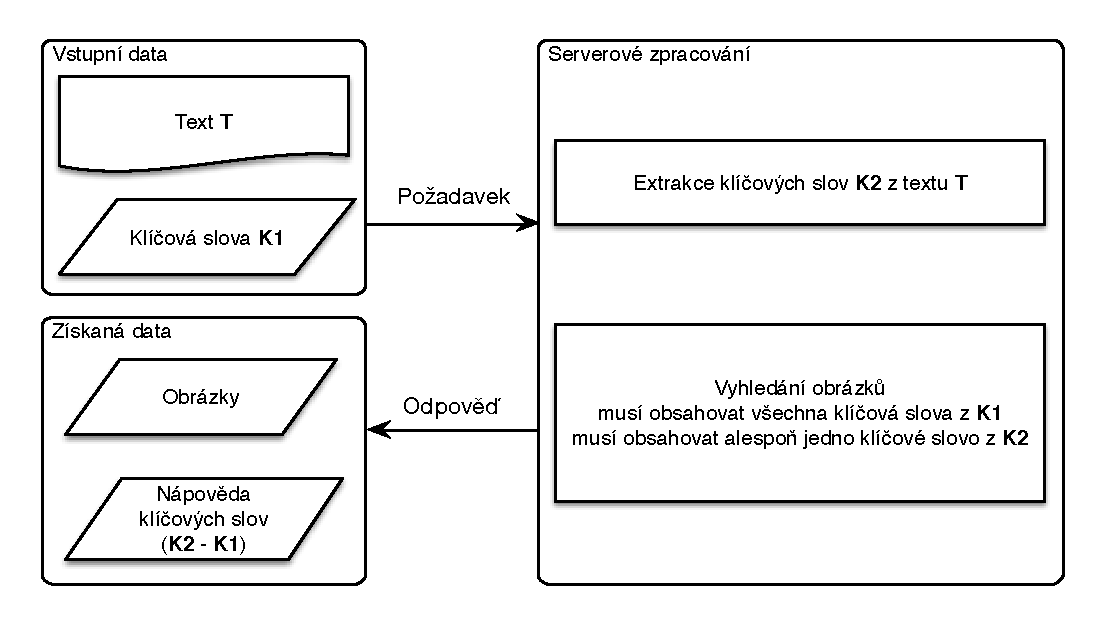
\includegraphics[width=150mm]{dataflow.eps}
  \caption{Základní tok dat mezi klientem a serverem.}
  \label{fig:dataflow}
\end{figure}


Aplikace poskytuje uživateli dvě možnosti vyhledávání. Základní uživatelským scénářem je vložit do rozhraní text. Aplikace by v takovém případě měla poskytnout relevantní obrázky k danému textu. V dalším uživatelským scénářem je přímý požadavek na klíčová slova obrázku. Uživatel by měl mít možnost zadat přímo klíčová slova, které nalezené obrázky musí obsahovat. Oba scénáře by mělo navím být možné propojit pomocí nápovědy klíčových slov -- uživatel zadá do rozhraní text, dostane výsledné obrázky a nápovědu klíčových slov, kterými může množinu nalezených obrázků více omezit. Klíčová slova ze vstupního textu se dále používají jako nápověda uživateli, který jimi může množinu hledaných obrázků dále omezit. Celý proces hledání vhodných obrázků popisuje diagram \ref{fig:dataflow}.



\section{Extrakce klíčových slov}

Extrakce klíčových slov je velmi důležitou složkou celého vyhledávání. Článek \cite{lott} shrnuje základní techniky extrakce klíčových slov z textu. Algoritmy na extrakci klíčových slov lze v zásadě rozdělit do dvou kategorií - \uv{s korpusem} a \uv{bez korpusu}. Metody pracující bez korpusu jsou zajímavé a mohou dosahovat podobných výsledků jako metody s korpusem. My však máme k dispozici dataset Profimedie, takže o metody pracující bez korpusu se tato práce dále nezajímá. 

\subsection{TF-IDF}

TF-IDF je jeden ze základních vyhledávacích algoritmů. Algoritmus využívá korpusu dokumentů $D$ a dvou složek $TF$ a $IDF$, lze ho vyjádřit jako rovnost: 

\begin{equation}
  TFIDF(t,d,n,N)= TF(t,d)\times IDF(n,N)
\end{equation}

Složka $TF$ znamená $TERM\ FREQUENCY$ a pokud $t$ je slovo a $d \in D$ je dokument, je $TF$

\begin{equation}
 TF(t,d) = \sum_{slovo\,\in\,d} \begin{array}{l l} 1 & \mathrm{pokud}\ slovo = t \\
  0 & \mathrm{jinak} \end{array}
\end{equation}

Jedná se tedy o frekvenci slova v dokumentu.

Složka $IDF$, tedy $INVERSE\ DOCUMENT\ FREQUENCY$ vyjadřuje, jak moc daný termín popisuje dokument. Pokud je $N$ počet všech dokumentů v $D$, tedy $N = |D|$ a $n$ je počet dokumentů, ve kterých se vyskytuje slovo $t$, je $IDF$ tohoto slova

\begin{equation}
IDF(n,N) = \log \left(\frac{N}{n}\right)
\end{equation}

\begin{equation}
IDF(n,N) = \log \left(\frac{N - n}{n}\right)
\end{equation}

Čím je tedy slovo v korpusu častější, tím více se s logaritmem snižuje jeho informační hodnota. Slova, která jsou velmi běžná většinou klíčovými slovy nejsou.

Výsledný vzorec pak jde shrnout jako:

\begin{equation}
TFIDF(t,d,n,N)= \left(\sum_{slovo\,\in\,d} \begin{array}{l l} 1 & \mathrm{pokud}\ slovo = t \\
  0 & \mathrm{jinak} \end{array}\right)
  \times
  \log \left(\frac{N - n}{n}\right)
\end{equation}

\subsection{TF-IDF pro extrakci klíčových slov}

Algortimus TF-IDF můžeme použít pro extrakci klíčových slov z textu. Všechna znaky vstupního textu převedeme na malá písmena a text rozdělíme na slova. Dále nás nezajímá diakritika a různé speciální znaky, které může text obsahovat. Všechna slova převedeme na stemy. O převodu slov na stemmy se podrobněji píše v Kapitole \ref{chap:stemmer}.



Problémem tohoto algoritmu pro je odlišný charakter korpusu a vstupních dat. Vstupní data jsou typicky novinový článek. Pokud bychom jako korpus použily anotované obrázky, získáme špatné výsledky. Běžná anglická slova, jako "the", nebo "a" se v takovém korpusu vyskytují velmi zřídka, jejich IDF tedy bude vysoká. Naopak TF v běžném novinovém textu je vysoké. Takovýto korpus nám pak označuje jako klíčová slova běžná anglická slova.


\subsection{Extrakce bez korpusu}

Dalším druhy algoritmů ke své práci korpus nepotřebují a pracují pouze se vstupním textem.

\section{Řešení: jaké algoritmy zvoleny, získání tréninkových dat}

Jako nejvhodnější řešení byl nakonec zvolen TF-IDF algoritmus. Jako kandidáti jsou odfiltrována slova, která se nenacházejí v datech Profimedie. Jako korpus k měření IDF byla použita data článků z Wikipedie.

Pro rychlé testovací účely bylo oanotováno pár článků z anglických wikinews. V každém článku jsem označil pět klíčových slov. Porovnávání algoritmů na extrakci klíčových slov pak vzalo pět nejpravděpodobnějších klíčových slov podle algoritmu a porovnalo v kolika procentech se algoritmus trefil s anotací.



